\documentclass{ctuthesis}
\ctusetup{
    xdoctype = B,
    xfaculty = F3,
    mainlanguage = english,
    titlelanguage = english,
    title-english = {Model of CAN FD Communication Controller for QEMU Emulator -- Analysis, Transmission and Reception},
    title-czech = {Model kontroléru CAN FD v emulátoru QEMU -- analýza, vysílání a příjem},
	doctype-english = {Bachelor Thesis},
    department-english = {Department of Control Engineering},
    author = {Jan Charvát},
	keywords-czech = {CAN bus, CAN FD, QEMU, Linux, CTU CAN FD, SocketCAN},
	keywords-english = {CAN bus, CAN FD, QEMU, Linux, CTU CAN FD, SocketCAN},
    supervisor = {Ing. Pavel Píša, Ph.D.},
    supervisor-address = {Praha 2\\ Karlovo náměstí 13\\ E-7a},
    month = 5,
    year = 2020,
}
\ctuprocess
\usepackage{tabularx, array, booktabs}
\begin{declaration}
Prohlašuji, že jsem předloženou práci vypracoval samostatně, a že jsem uvedl veškerou použitou literaturu.

V Praze, 17. ledna ~\ctufield{year}
\end{declaration}
\begin{thanks}
I would like to thank Ing. Pavel Píša Ph.D for tutoring and time investments towards my Thesis.
\end{thanks}
\begin{abstract-english}
 This thesis begins with a theoretical part, where is an analysis of CAN 2.0 and differences with newer standard CAN FD. It continues with QEMU CAN subsystem discovering. As a practical part is an implementation of CAN FD communication bus and emulation of CAN FD capable chip as an extension of already implemented CAN 2.0 capable chip SJA1000.
\end{abstract-english}

\begin{abstract-czech}
 Tato práce začíná teoretickou částí, kde je analýza CAN 2.0 a rozdíly s nevějším standardem CAN FD. Ta pokračuje s objevováním CAN subsystémů v QEMU. Jako praktická část je implementace CAN FD komunikační sběrnice a emulace čipu uzpůsobeného pro CAN FD jako rozšíření již implementovaného CAN 2.0 čipu SJA100.
\end{abstract-czech}

\begin{document}

\maketitle
\chapter*{Nomenclature}

\noindent
\begin{tabularx}{\linewidth}
  { l >{\raggedright\arraybackslash}X }
\bfseries Acronym  & \bfseries Meaning \\\Midrule
CTU & Czech Technical University \\
CAN & Controller Area Network \\
FD & Flexible Data Rate \\
ECU & Electronic control unit \\
PCI & Peripheral Component Interconnect \\
CANH & CAN-Hight line \\
CANL & CAN-Low line \\
SOF & Start of Frame \\
RTR & Remote request \\
IDE & Identifier Extension bit \\
DLC & Data Length Code \\
CRC & Cyclic redundancy check \\
ACK & Acknowledgement \\
BRS & Bit Rate Speed \\
FDF & Flexible Data Rate Frame \\
ESI & Error Status Indicator \\
Tx buffer & Stores the data for transmission \\
Rx buffer & Stores the received data \\
TXCE & "set\_empty" command \\
TXCR & "set\_ready" command \\
TXCA & "set\_abort" command \\
RXFRC & RX buffer frame count \\
RWCNT & Count of words in CAN frame without FRAME\_FORMAT WORD \\
\end{tabularx}

\chapter{Introduction}
 This bachelor thesis goal is to implement CAN FD communication bus and controller emulation for QEMU full system emulator mode. It builds on previous and ongoing CAN bus related projects developed and or coordinated by CTU FEE. The support of the classic SJA1000 CAN 2.0 controller model for QEMU emulator development started by Jin Yang in RTEMS GSoC 2013 slot mentored by Pavel Pisa from CTU and reached QEMU mainline in 2018. \cite{qemu-mainline} CTU CAN FD controller \cite{ctu-canfd-core} initiated by Ondrej Ille at CTU FEE is selected as the device model used by a guest system to access the CAN FD bus variant. Linux kernel driver for this controller is available as the result of Martin Jerabek's theses. \cite{ctu-canfd} \\
 The CAN controller core emulation needs to be connected to some system bus to be visible by emulated CPU and the guest system. The model of commercially available Kvaser PCI addon card is used for the SJA1000 emulation. The PCI Express card integration of CTU CAN FD is available as the project. \cite{ctu-project} \\
 SocketCan is used to interface QEMU emulated CAN bus to the CAN bus of the host system when QEMU is run on the Linux system. The QEMU side of the interface has to be extended to support CAN FD protocol.
 The most significant implementation part of this project is to emulate CTU CAN FD IP Core register map \cite{progdum} with QEMU and get communication through this emulated hardware parts on a real CAN hardware bus and see this communication on the other side by monitoring tools. \\
 This project is open-source the same as the whole QEMU. \\
 My focus to CAN bus is a result of participation in one external company
 project, which delivers utility for a train where CAN communication is used.

\chapter{CAN}
 Automotive industry often uses CAN.  For instance, almost every car uses CAN bus. One of the reasons is the need not to carry hundreds of kilograms of wire in the car. CAN enable the connection between several ECUs via one bus\cite{ECUs} instead of many analogue signal lines. Next advantage is that all nodes receive each message and decide if they want to use it or not. However, the application spectrum is broad. CAN standardised Bosch company in 1986. Hence make industry needs and CAN development significant progress. This bachelor thesis aim to the last most significant innovation CAN FD.

 \section{CAN 2.0}
  ISO 11898-1:2003 describes CAN 2.0. In the picture is a visible frame bit after bit. If it is to be sent 8 bytes data, it is visible a quite significant overhead. 
  \begin{figure}[H]
  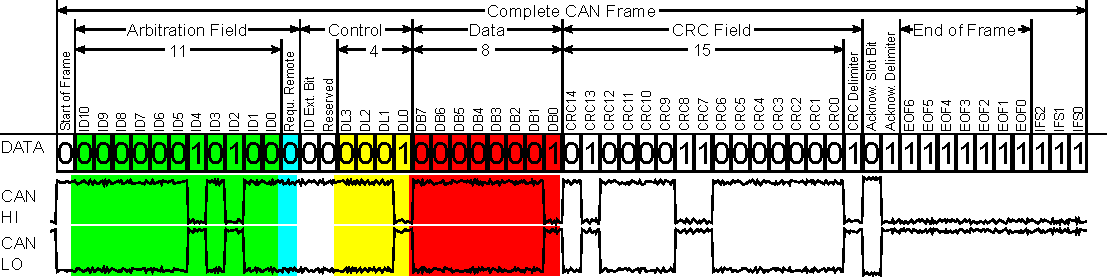
\includegraphics[width=1\textwidth]{CAN-Bus-frame_in_base_format_without_stuffbits}
  \caption{CAN frame detail \cite{can_frame}}
  \end{figure}
  The frame starts with SOF, which is always dominant zero. It serves to notify other CAN nodes at the beginning of the arbitration on the sending of a new frame. Then comes identifier, CAN 2.0 brings two length variants for ID, CAN 2.0a corresponds with a sample image and has an 11-bit identifier. CAN 2.0b standard extends identifier to 29-bit. RTR in dominant zero marks standard frame, in the recessive state it changes into a Remote frame, which requests for data from a CAN node with the corresponding ID assigned to the identifier place. IDE distinguished between standard and extended ID format. DLC holds data bytes count that is number between 0 to 8 bytes per message, then come the data. CRC is for data integrity check. ACK first bit is space for confirmation that at least one CAN node accept the message and the second bit for information that at least one CAN node has not accepted the message correctly. If the second condition is accomplished, the whole frame is resent automatically.
  \subsection{Physical layer}
   CAN physical layer consist of twisted pair cabling CANH and CANL. Logic value is counted as a result of CANH - CANL and is called Vd\cite{can_Vd}. Exact limiting values generally differ, but when both wires have similar voltage - Vd is close to zero, it is logic 1, and both wires are in recessive state. Dominant state means that in CANL decreased voltage and in CANH increased voltage, Vd gets over a specific limit into logic 0.
  \subsection{Transmission priority}
   CAN node priority depend on its ID, which must be unique across the bus. In the case, when more CAN nodes want to transmit data, arbitration wins the CAN node with the lowest ID. It means that can bus transmission is priority-based, and the highest priority is a CAN node with ID full of zeros. The reason comes from the physical layer, the transmission of the identifier is bitwise, and logical zero on the bus means a dominant state. Therefore, if the current's CAN node identifier contains 1, it wants to change the transmission to a recessive state. However, the dominant state representing a logical zero remains on the bus, the current CAN node realises that somewhere across the bus is also transmitting a CAN node with a higher priority, so this CAN node stops transmitting and switch to receive mode only and waits until next arbitration.
  \subsection{Bit stuffing and CRC}
   The final frame, which is sent through the bus, is not always fixed length because of the bit stuffing. This algorithm adds a different bit after five times repeated bit of same value. These redundant bytes relate to synchronisation algorithm because CAN bus does not have fixed timer authority. These bits could be added between SOF and the end of the  CRC and are not counted by CRC\cite{can_crc}.

 \section{CAN FD}
  CAN FD extends the original CAN with the flexible data rate, it means that data could have a higher bit rate than the rest of the frame. It is necessary to keep a slower bit rate for the identifier due to the arbitration principle of selecting the highest priority CAN node\cite{priority_can}. Bit rate speed in the automotive industry is about 500 Kbit/s for the arbitration phase and 2 Mbit/s or more for the data phase\cite{canfd_calculator}. In CAN FD also increases maximum data length from 8 bytes to 64 bytes. All mentioned above describes ISO 11898-1:2015.
  \begin{figure}[H]
  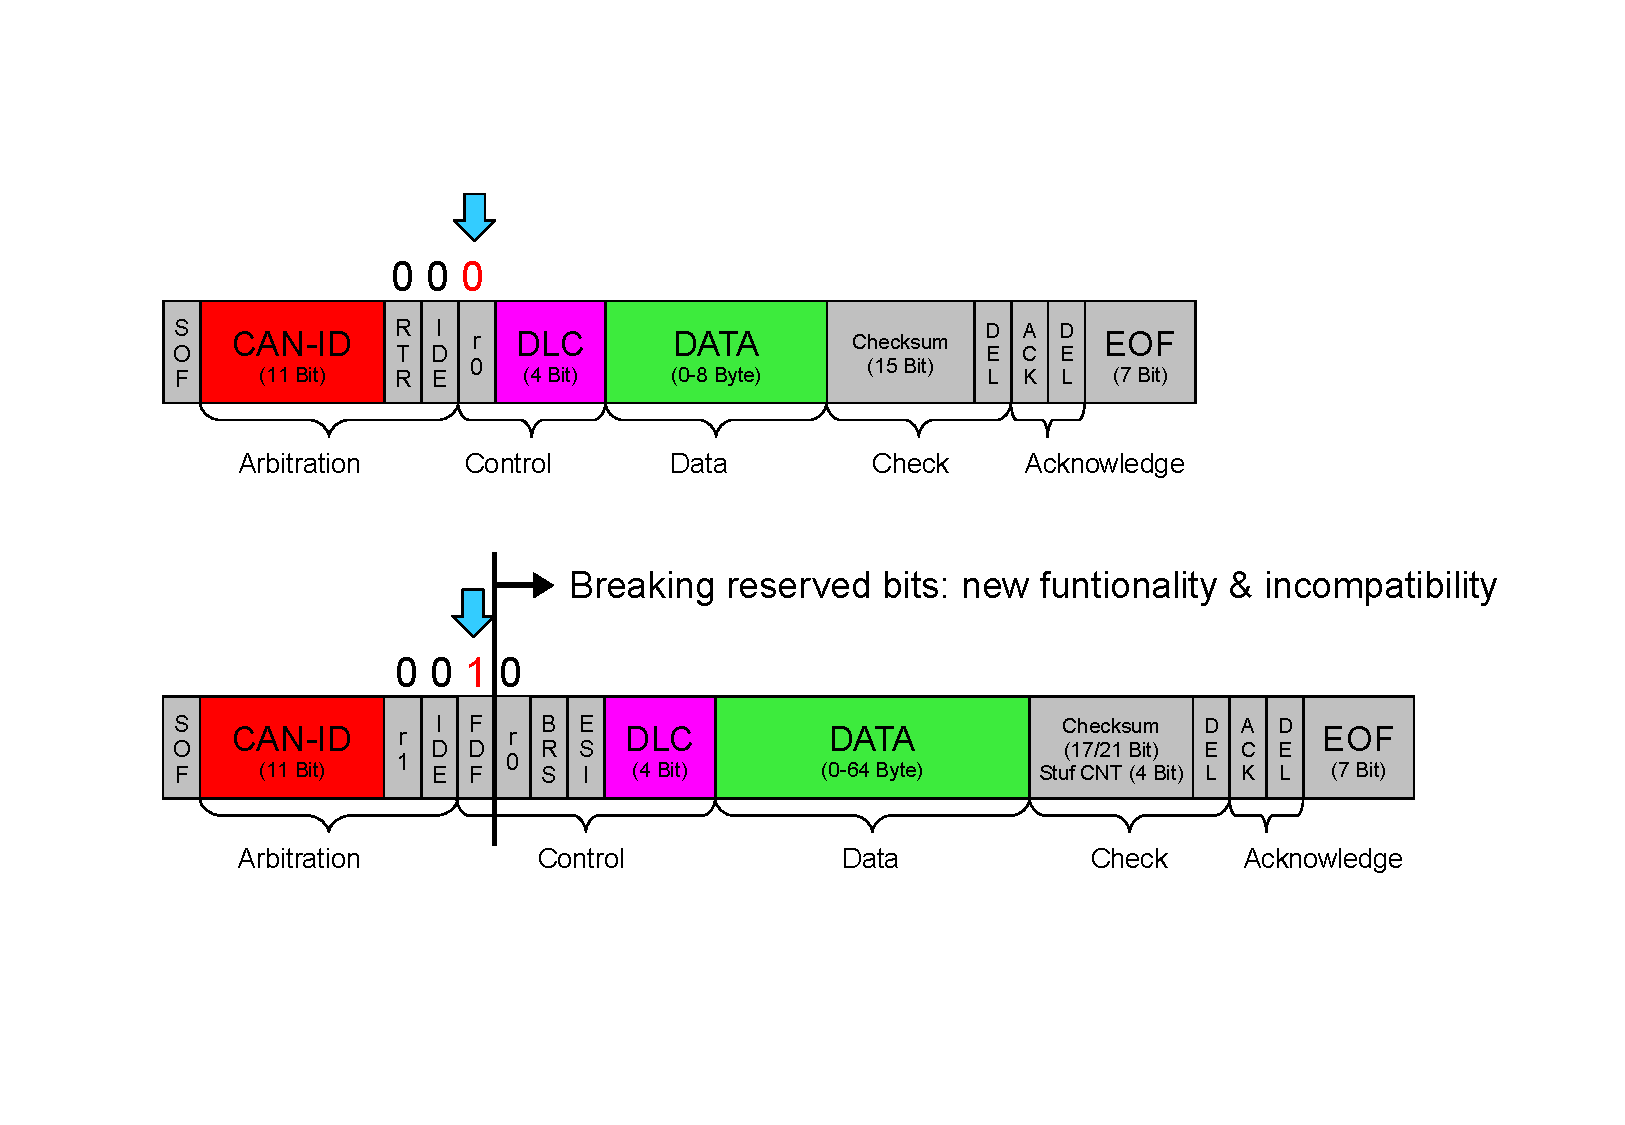
\includegraphics[width=1\textwidth]{agl2017-socketcan-can_fd}
  \caption{CAN and CAN FD difference \cite{canfd}}
  \label{fig:cancanfddifference}
  \end{figure}
  \subsection{Compatibility}
  \label{section:combability}
   There is no direct compatibility between CAN and CAN FD due to changes in the control field, see Figure ~\ref{fig:cancanfddifference}. Inconsistency appears in a reserved bit, which is for CAN 2.0 always dominant 0, but now transforms into FDF flag indicating CAN FD frame. Classic CAN 2.0 controller would not recognise CAN FD frame and reject an error frame. Three new bits have been added into the control field. Reserved bit has been added for a possibility of future extension with a new protocol, BRS in recessive 1 indicates a faster bit rate shift of data phase and ESI informs about error passive - logic one or error active transmitter state.
   \subsubsection{Bit stuffing and CRC}
    Condition for bit stuffing has been changed. Stuff bits could be added between SOF and newly at the end of the data field with the same principle as CAN 2.0. CRC now counts with these stuffed bits. Stuff bits are also added in CRC but have modified principle. CRC has been improved because several bits have been added and newly has not always the same length. In the checksum is stuff bit count to support CRC with data integrity.
   \subsubsection{Data length code mapping}
    One of the most significant difference is a DLC field, which holds an individually coded length of the data. Data of arbitrary length up to 64 bytes integrate into one of the possible intervals. First 8 bytes correspond with standard CAN frame and continue with 12, 16, 20, 24, 32, 48 or 64 bytes length. This non-linear ordering is due to historical reasons that only 4 bits are available.
    \begin{figure}[H]
    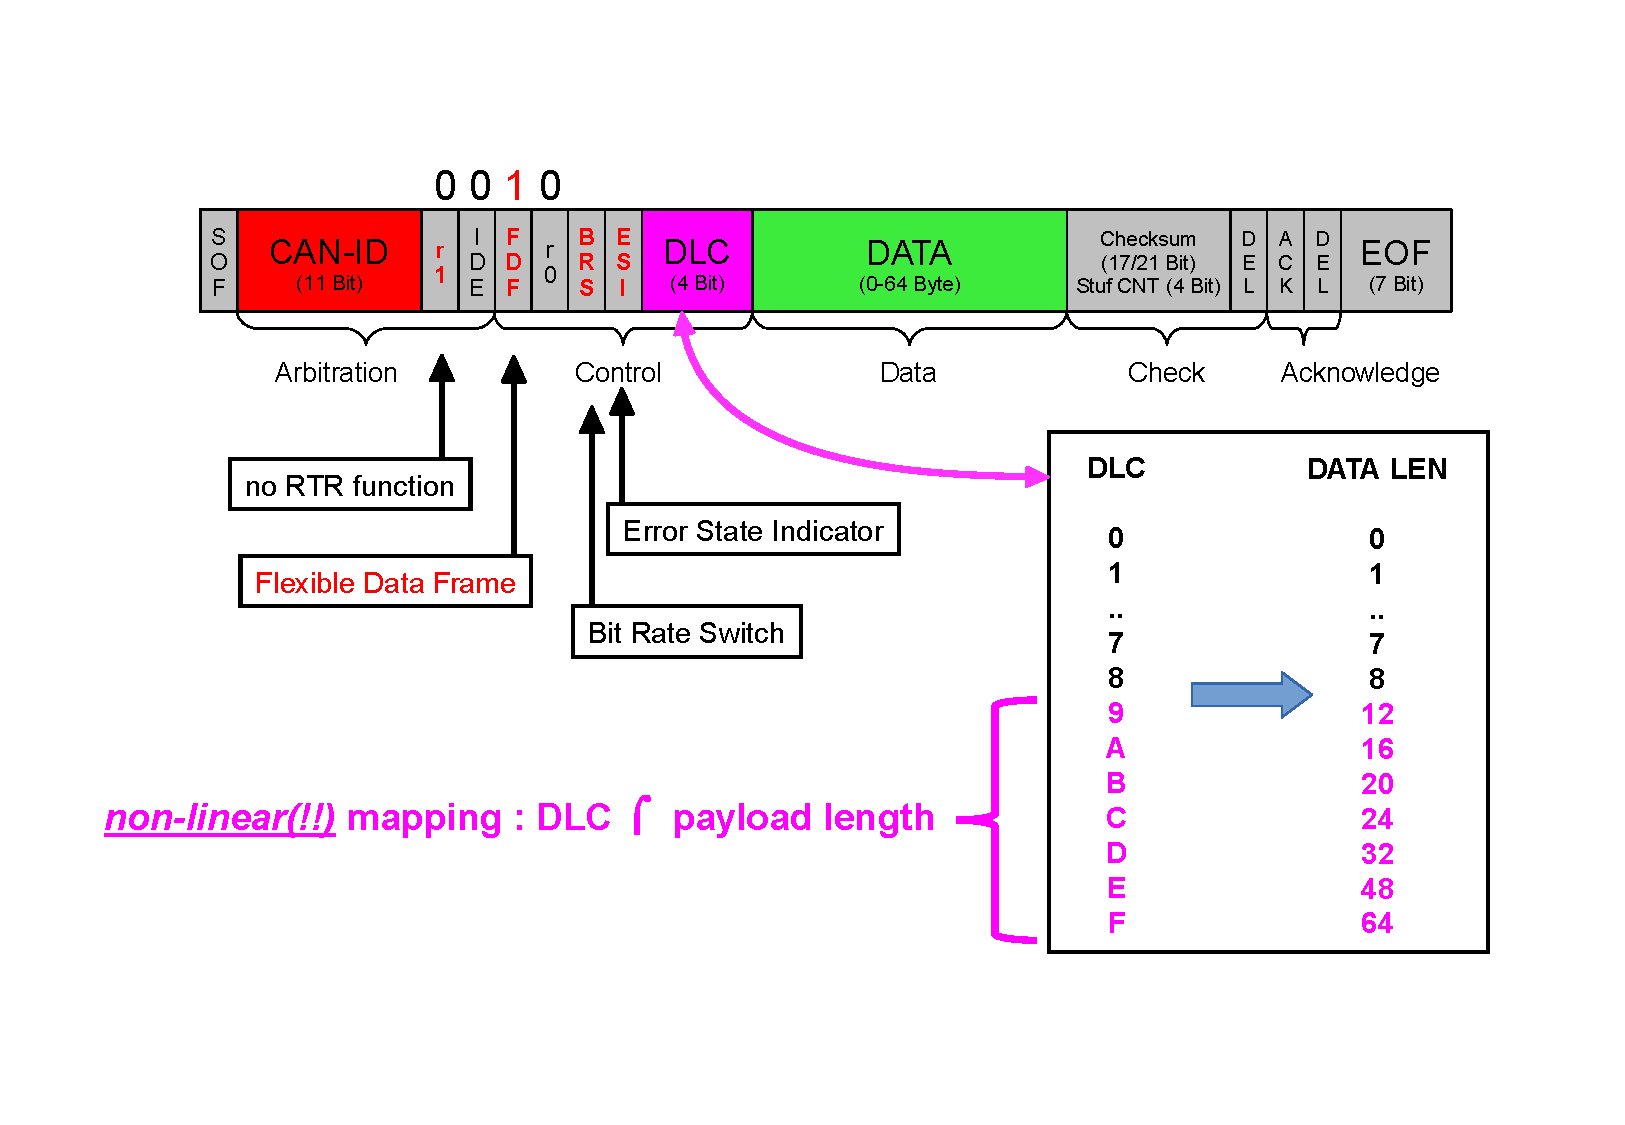
\includegraphics[width=1\textwidth]{agl2017-socketcan-can_fd_dlc}
    \caption{CAN FD frame DLC table \cite{canfd_dlc}}
    \end{figure}
 
\chapter{QEMU emulator}
 QEMU is a universal virtualisation tool because of several modes for working. The original purpose was to launch processes compiled for another architecture without the need to change current architecture (ARM, MIPS, Linux). However, it is used today more often for full system virtualisation including peripherals virtualisation. Support to the CAN bus and controllers emulation has already been accepted into mainline. Nevertheless, CAN bus standard evolves, and a new extended variant of the protocol was introduced in 2012. It is called CAN FD to highlight the use of higher bit rate for the data portion of the frame.

 \section{Automated testing}
 Linux is already able to handle CAN FD communication, even create virtual CAN bus and set up communication there. A problem occurs with a new CAN interface driver development or implementation of a driver for another operating system. Most project maintainers want to be able to test automatically new changes without all the hardware. It is one of the reasons why started the integration of virtualisation of the CAN bus into QEMU\cite{qemu_development}.

 \section{QEMU Object Model}
  The newest QEMU device model consists only of devices and properties\cite{qemu_qom}. Properties are the external interface to an object. That means it is different from previous Qdev separation for devices and busses. New device creation is initialised with properties set to default values and has no parent. Each device has a unique name, derived from the parent name.

 \section{QEMU architecture}
  Image bellow well describes emulation inside QEMU, and quite good explanation is in CAN support to QEMU emulator documentation. \cite[page 2-4]{qemu-mainline}
  Linux mainlined Socket CAN API was selected as a connection between host - real CAN hardware and guest system running QEMU with virtualised CAN devices. Each virtual CAN device is seen as a PCI device by the guest system.
  Two or more emulated controllers could be connected and create virtual CAN bus, and this communication will be visible only in QEMU. One or several interfaces could be connected to the host system via SocketCan and will be observable in the host system by monitoring tools. It is necessary to connect only one controller to the host system. Otherwise, an infinite loop occurs.
  \begin{figure}[H]
  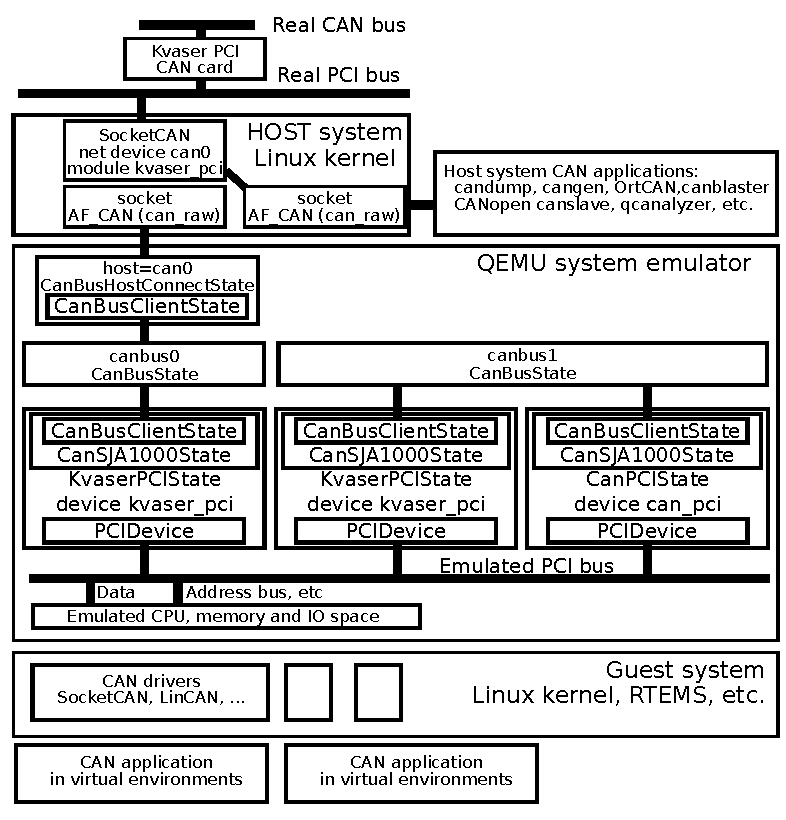
\includegraphics[width=1\textwidth]{qemu-can-bus}
  \caption{QEMU system emulator \cite{qemu-canbusexplain}}
  \end{figure}
 
 \section{QEMU CAN subsystem}
  To be able to access CAN bus in Linux, a physical card is required. Then a driver must be implemented, which understands the data sent over the bus. 
  The emulated controller SJA1000 is I/O mapped to a single region of emulated Kvaser PCI CAN card. Reading and writing to this region is directly map to SJA1000 chip read or write operations, which supports only byte size access.
  QEMU also should be able to freeze, save the whole state into prepared VmDescription structures and migrate to another computer, even to another architecture.

 \section{Coding style}
  QEMU coding style \cite{qemu-style} is similar to the recommended Linux kernel style \cite{linux-style}. In QEMU repository is the script which checks the written code and shows all problems. The most common mistakes are tabs instead of 4 spaces, spaces or tabs on an empty line, wrong using of parenthesis.
 
\chapter{Implementation}
 As the next part of this bachelor thesis is the implementation of CAN FD capable chip, which will support QEMU CAN subsystem. Fundamental abilities have been implemented, such as transmission and reception. 
 \section{Integration}
  It is necessary to extend QEMU side SocketCan interfacing because it accepts only CAN 2.0 messages. SocketCan has been adopted from the Linux kernel. Therefore, it is possible to be inspired there to expand the support of CAN FD. When the bus enables frames of CAN FD standard, it necessary two thigs to happen. Firstly must be SJA1000 chip slightly modified to be CAN FD tolerant and do not generate error frames. As the next part of CAN FD integration, CTU CAN FD PCI card based on Kvaser PCI CAN card emulation implemented by Jin Yang and Pavel Pisa has to add. Last implementation goal is an emulation of CTU CAN FD IP CORE as a controller mapped into CTU CAN FD PCI card.
 \subsection{SocketCan support for CAN FD}
  Initial host SocketCan support has been added for CAN FD. SocketCan subsystem allows sending and receiving from the CAN 2.0 controller. CAN FD frames handling requires to send structure with differences in memory size to SocketCan file handler. Struct qemu\_can\_frame has been extended to hold a more extended data field. On top of that property called flags has been added into message structure. Property called flags is uint8\_t and holds added bits by the new standard such as BRS, ESI and FDF, see~\ref{section:combability}. Property DLC remains same, but in CAN frame are stored accurate data bytes count instead of DLC code, because it simplifies the kernel's back-checking for record lengths.

 \subsection{CTU CAN FD core support}
  Initial CTU CAN FD core support has been started as a copy of SJA1000. Right at this moment is only SJA1000 chip controller supported. Therefore starts the creation of CTU controller supporting Can FD.
  When CTU CAN is integrated into a PCI Express board, then two BARs (Base Address Regions) are expected by the driver. The first keep value to identify the CAN core and provides a number of integrated core instances in the other region. The second region maps registers of the core instances one after another. The registers to control PCI Express MSI (Message Signaling Interrupts) and other FPGA chip-specific control functions are mapped at some offset to the first region as well. At the beginning of the work, it is focused on the critical registers for transmission and reception. Except control registers must be implemented correct behaviour of access for four TX buffer and cyclic FIFO RX buffer. Then are implement less important read/write registers, for sample traffic counters or controller state diagnostics.
 
 \subsection{Registers emulation}
  CTU CAN FD core register definitions by Ing. Ondrej Ille has been used. It is a significant amount of memory mapping structures, precisely unions, which defines the layout of bits in registers in real hardware. It distinguishes between several types of bits in hardware registers, read-only, write-only or read/write bits. Everything is in product documentation, and it is necessary to follow it for correct emulation behaviour. The documentation describes the functional description of CTU CAN FD, programmers model, and parameters of CTU CAN FD. To correct chip emulation must be each bit correctly handled. To access CTU CAN FD device data is possible only through individual registers, it means memory access aligned to words. To be able to read or write, it is necessary to call read or write function with the correct address of the required register as a parameter.
  Control registers have several functionalities. Write only commands to change inner state, status information about internal traffic counters, errors report and so on or reading of received data.
 
  \subsubsection{Data structures}
  The internal state of CTU CAN FD controller must be saved somehow. CTU CAN FD core register definitions
 
 \subsection{Interrupts}
 
  \subsubsection{Interrupt mask}
  
  \subsubsection{Invoke interrupt}
 
 \subsection{SJA1000 CAN FD tolerant}

 \section{Transmission}
  TX buffers are used for transmission by CTU CAN FD. They are filled by software, which knows the mapping of TX buffers and stores word after word whole frame. When the whole frame is stored into arbitrary Tx buffer, Tx command TXCR is set. During the processing of TXCR command, it means writing to exact register, controller set buffer into the READY state and immediately sends the frame and change buffer state into buffer OK state. There is no implementation of delay yet. It follows that the transmission cannot be aborted. During this procedure, all Tx buffers are iterated, and Tx buffer in the READY state, which corresponds with the flag of the related buffer is sent.

 \subsection{TX buffers}
  Initial implementation of TX buffers is 0x50 bytes uint\_8t array, computed to be just enough for the maximum size of CAN FD frame. Four Tx buffers are in CTU CAN FD prepared for the transmission. Support of transmission buffers is necessary for correct message sending. Buffer with a stored whole frame inside is transmitted to the bus. Then informs through interrupt requests that transmission took place and that at least one buffer is again in OK state.

  \subsubsection{Buffer states}
  The initial state for all four buffers is the EMPTY state. It indicates that a buffer is free to be used. Same meaning has the OK state, which is set after successful transmission. When the data are ready to be sent, it is the READY state. The ABORT state is not implemented due to no transmission delay, the same for the FAILED state. The FAILED state occurs when several unsuccessful attempts are made.
 
 \subsection{Commands}
  Several Tx commands are defined. TXCE is able to reset buffer state to initial state. This command could change the FAILED state buffer back to functionality, also affects the OK state and the ABORTED state. TXCA changes the READY state into the ABORTED state. Theoretically, it is possible, but transmission delay is not implemented, so it is not possible to reach this command functionality. The most important command TXCR sends a frame to the bus. Simultaneously set the OK state, the FAILED state or the EMPTY state to the READY state.
 
 \subsection{Buffer to frame}
  Before sending any data to the bus, it is necessary to move them from an internal stored buffer - this format is defined the same way as the CTU CAN FD core register definitions - to a generally understandable SocketCan frame format. First is an initialisation of QEMU CAN frame structure, data are loaded from the internal buffer by mapping unions which enables to copy the correct bits. At the end of the process, it is possible to directly memcopy the data phase. Every frame stored in Tx buffer is stored there according to the same rules, so header has always 16 bytes and maximum of the data phase could be 64 bytes.
  memcpy(frame->data, buff + 0x10, 0x40);
 
  \subsubsection{DLC to length}
   Real bytes count is encoded by CAN FD standard into DLC. It is necessary to take care of this non-linear mapping because in the internal buffer is DLC stored by CAN FD standard, but in the frame, which would be sent to the bus is required to hold in DLC real bytes count, because it simplifies the kernel's back-checking for record lengths. Non-linear mapping solution could be found in can\_emu.h as dlc2len function. A little problem is with identifier because it is in the frame as one number, but in defined internal buffer layout, it is divided to the base and extended identifier. The solution is simple, in case of using the only base identifier, the base identifier is assigned to CAN ID. In the opposite case, the extended identifier is assigned first and then use logical OR to add the base identifier shifted by 18 to the left. 
   
 \section{Reception}
  Reception is implemented through single FIFO organised Rx buffer. All incoming messages from the bus are stored one after each other. Reading from Rx buffer is going through RX\_DATA register. CTU CAN FD is able to recognise the first and the last word of the frame in the Rx buffer. When the whole frame is read by software, can continue next frame reading immediately.

 \subsection{RX buffer}
  Rx buffer is uint\_8t array with an arbitrary length. After each reception is RXFRC updated. Several messages can be stored during the usual system running, therefore occurs a need for orientation during words reading by SW. This is the reason why the CAN frame reminder was created. After check that Rx buffer is not empty, CAN frame reminder appears as an essential element. If CAN reminder is zero, we read the first word of the new frame. By frame alignment definition is possible to mapped correct structure on it and read RWCNT from which is length of the frame calculated.
 
  \subsubsection{FIFO implementation}
   There are several possibilities of how a FIFO  could be implemented. For data reading per bytes, is very often used a tail pointer. Head pointer is also essential but is used only for storing the whole frame. Instead of the head pointer was decided to store accurate bytes count in the Rx buffer, from which is the head pointer easy to calculate. Accurate bytes count occurs in several conditions through CTU CAN FD.
 \subsection{Commands}
 
 \subsection{Frame to buffer}
 
  \subsubsection{Length to DLC}
   Before the incoming frame is possible to store into Rx buffer, it is necessary to move them from a generally understandable SocketCan frame format to an internal stored buffer - this format is defined the same way as the CTU CAN FD core register definitions. It is pretty similar to DLC to a length, but this time with one change. There is an urgency to count bytes in the frame correctly because it is used later for copying from a temporary buffer into the Rx buffer. 
  
 \section{Hardware Reset}
  A hardware reset is called in two cases, always after CTU CAN FD power-up or could be called through writing logic 1 to control register MODE flag RST. After power-up, the reset is more likely used to set up correct reset values. A more complicated situation occurs during a reset in the middle of work. In addition to setting the reset values, the work in progress must be cleaned up. Reset traffic counters, status control registers and interrupts. Each Tx buffer should return in the empty state. It is also necessary to flush Rx buffer. It contains several steps, reset tail position pointer, buffer bytes count and for a case of reset during frame reception also frame reminder.
 
\chapter{Testing}
 Necessary commands to prepare the testing environment and check the functionality of written code if data go through, messages identifications correspond.
 \begin{verbatim}  cd mnt/shareddir/bin/
  cd ~/QEMU_PATH/shareddir/bin\end{verbatim}
 These are paths to shared memory for communication between inner and outer Linux systems during QEMU emulation. It is possible to add files or binaries into the emulated system during its run. The first one is a command of getting inside the emulated system to the right directory. The second one is the directory accessible from the outer system.
 \begin{verbatim}  modprobe ctucanfd_pci
  ip link set can1 type can bitrate 1000000 dbitrate 1000000 fd on
  ip link set can1 up
  cangen can1 -f\end{verbatim}
 Sequence for testing purpose. Load CTU CAN FD module into the Linux kernel, set up a virtual CAN interface and run
 \begin{verbatim}  ~/QEMU_PATH/scripts/checkpatch.pl ctucan_core.c\end{verbatim}
 Check script for correct code style.
 \begin{verbatim}  candump [can0]
  cangen  [can0]
          [-f] CAN FD frames\end{verbatim}
 Necessary tools to display, record, generate and test CAN traffic. \cite{can-utils}
 \begin{verbatim}  test-ctucan -p -T -I 0x123 -f -b\end{verbatim}
 Send CAN frame with additional settings and debug output.

 \section{Actual testing environment setup}
  This bachelor project develops on the system with Windows 10 where it runs utility for virtual machines VMware  Workstation 15 player in its free version in non-commercial use only. \cite{vmware} \\
  On VMware run virtual machine Ubuntu 18.04.3 LTS, \cite{ubuntu} inside Ubuntu take place whole work with QEMU. QEMU also use virtualisation, so during the work, for testing purpose, the next Linux system emulates inside the QEMU and results in virtualisation chain, which is not the best practice for working, but luckily, it is possible. In this case, QEMU uses the same build of the Linux kernel as an external system. It means Ubuntu 18.04.3 LTS. QEMU is possible to run with -nographic parameter, and it uses the current terminal window as its native console. \\

 \section{Test SW}
 
 \section{Driver}
 
\chapter{Conclusion}

 \section{Work already completed}
  This project analyses the basic QEMU concept and how to work with it as a full system emulator. Also shows proper coding style for QEMU.  Next part analyses CAN frames differences between standards to be able to understand which parts changed and how to implement them. It is necessary to know the role of each bit of CAN frame to be able to handle them. The analysis brings a group of often-used commands which helps with the workflow or with the testing.
 
 \subsection{Transmission and reception}

 \section{Implementation}
  Already working emulation of CAN bus and stand-alone SJA1000 controller support has been extended, CAN FD support has been added and now is CTUCAN FD core controller available with modified card CTUCAN PCI. Nowadays, the transmission of CAN FD frames is available. The new implementation keeps previous functionality of sending CAN 2.0 frames.

 \subsection{Future implementation goals}
  Consider messages rate slowdown as on real CAN bus. Some mechanism prevents to some limit lost of messages when a guest application is slow. Convert CAN bus model from plain C to QOM (Controllers are QOM/Qdev already). Add more CAN controllers model emulation (BOSCH/Ti C CAN, Freescale FlexCAN, etc.).
 
 \subsection{Transmission delay}
 
 \subsection{Vision}

\chapter{Attachment 1}
 
 \section{Installation guide for programmers}
  Check installation of git versioning system by
  \begin{verbatim}  git --version\end{verbatim}
  if there is no installation on computer write command
  \begin{verbatim}  sudo apt install git\end{verbatim}
  Now pull QEMU mainline from git
 \begin{verbatim}  git clone git://git.qemu.org/qemu.git\end{verbatim}
  Will continue with proper installation way. \\
  Until the project is not in mainline, it could be found here.
  \begin{verbatim}  git remote add gitlab-fel https://gitlab.fel.cvut.cz/canbus/qemu-canbus.git
   git checkout -b charvj10-canfd gitlab-fel/charvj10-canfd\end{verbatim}

\chapter{Attachment 2}

 \section{Useful commands}
  During the work is a great advantage to know some hidden features which are available on the actual system or program. It could make progress faster and simpler. A division between general Linux advice and specific testing purpose commands help with the problem understanding and shows personal usage what might do work easier.
 \section{Linux}
  For heavy Linux users are these commands and features natural, but for standard users, or mainly Windows programmers can help. The advice also contains shortcuts for Midnight Commander \cite{mc}. MC during the bachelor project proof itself as a great file explorer to browse and work with the file-system.
  \begin{verbatim}  F9 + cf\end{verbatim}
  MC F9 Command Find, go through the whole directory and try to find the written filename or keyword.
  \begin{verbatim}  lspci-full -v\end{verbatim}
  Display full information list about devices connected to the PCI bus.
  \begin{verbatim}  rdwrmem -b 4 -s 0x08010000 -l 100 -m\end{verbatim}
  Dump certain memory location. \cite{rdwrmem}
 
 
\renewcommand\bibname{References}
\begin{thebibliography}{1}
\bibitem{qemu-mainline} http://rtime.felk.cvut.cz/publications/public/rtlws2015-qemu-can.pdf
\bibitem{ctu-canfd-core} https://gitlab.fel.cvut.cz/canbus/ctucanfd\_ip\_core
\bibitem{canfd_calculator} CSS Electronics, CAN FD EXPLAINED - A SIMPLE INTRO: Efficiency and Avarage Bit Rates, https://docs.google.com/spreadsheets/d/\\16XIceuoG\_YBlgyFKXxjYQk2016ln3NeEC68yoMFvwkA/edit\#gid=0, accessed: 2020-05-17.
\bibitem{ctu-canfd} https://dspace.cvut.cz/bitstream/handle/10467/80366/F3-DP-2019-Jerabek-Martin-Jerabek-thesis-2019-canfd.pdf
\bibitem{ctu-project} https://gitlab.fel.cvut.cz/canbus/pcie-ctu\_can\_fd
\bibitem{progdum} http://canbus.pages.fel.cvut.cz/ctucanfd\_ip\_core/Progdokum.pdf
\bibitem{ECUs} CSS Electronics, CAN BUS EXPLAINED - A SIMPLE INTRO (2020), https://www.csselectronics.com/screen/page/simple-intro-to-can-bus/language/en, accessed: 2020-05-16.
\bibitem{can_frame} https://upload.wikimedia.org/wikipedia/commons/5/5e/CAN-Bus-frame/\_in\_base\_format\_without\_stuffbits.svg
\bibitem{can_Vd} Texas Instruments, Automotive Controller Area Network (CAN) Overview and Training, https://www.youtube.com/watch?v=YrJn2AyWVBc - time 4:40, accessed: 2020-05-16.
\bibitem{can_crc} Vector E-Learning, Introduction to CAN (EN), https://elearning.vector.com/mod/page/view.php?id=370, accessed: 2020-05-16.
\bibitem{priority_can} CSS Electronics, CAN FD EXPLAINED - A SIMPLE INTRO (2020), https://www.csselectronics.com/screen/page/can-fd-flexible-data-rate-intro, accessed: 2020-05-17.
\bibitem{canfd} Oliver Hartkopp, The CAN Subsystem of the Linux Kernel, https://wiki.automotivelinux.org/\_media/agl-distro/agl2017-socketcan-print.pdf by Oliver Hartkopp - page 49, accessed: 2020-04-01.

\bibitem{canfd_dlc} Oliver Hartkopp, The CAN Subsystem of the Linux Kernel, https://wiki.automotivelinux.org/\_media/agl-distro/agl2017-socketcan-print.pdf by Oliver Hartkopp - page 50, accessed: 2020-04-01.
\bibitem{qemu_development} RTEMS, QEMU with CAN Emulation, https://devel.rtems.org/wiki/Developer/Simulators/QEMU/CANEmulation, accessed: 2020-05-18.
\bibitem{qemu_qom} QEMU, Features/QOM, https://wiki.qemu.org/Features/QOM, accessed: 2020-05-18.
\bibitem{qemu} https://help.ubuntu.com/lts/serverguide/qemu.html
\bibitem{vmware} https://www.vmware.com/products/workstation-player/workstation-player-evaluation.html
\bibitem{ubuntu} https://ubuntu.com/download/desktop
\bibitem{qemu-canbusexplain} https://www.linuxdays.cz/2017/video/Pavel\_Pisa-CAN\_canopen.pdf
\bibitem{qemu-style} https://github.com/portante/qemu/blob/master/CODING\_STYLE
\bibitem{linux-style} https://www.kernel.org/doc/html/v4.10/process/coding-style.html
\bibitem{mc} https://midnight-commander.org/
\bibitem{rdwrmem} http://cmp.felk.cvut.cz/~pisa/linux/rdwrmem.c
\bibitem{can-utils} https://github.com/linux-can/can-utils/
\end{thebibliography}
\end{document}